\documentclass{article}
\usepackage{tikz}
\usetikzlibrary{arrows.meta,positioning,calc,shapes.geometric}
\pagestyle{empty}
\begin{document}
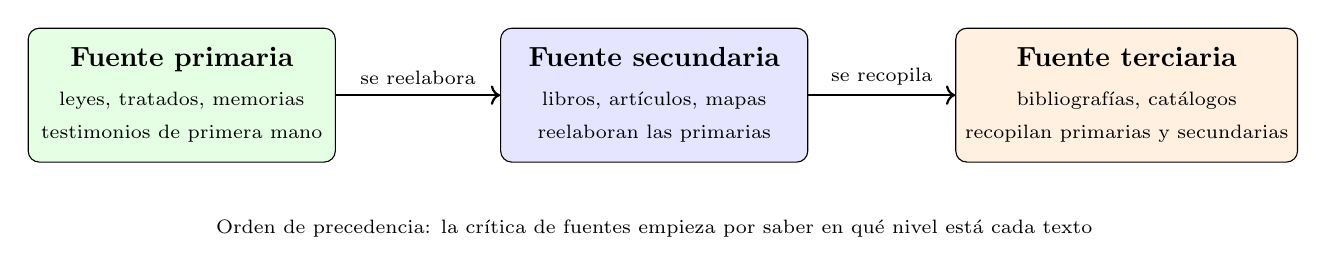
\begin{tikzpicture}
\tikzset{every node/.append style={align=center}}

\node[draw, rounded corners, fill=green!10, minimum width=3.9cm, minimum height=1.7cm, align=center] (p) at (0,0) {\textbf{Fuente primaria}\\[2pt] \scriptsize leyes, tratados, memorias\\ \scriptsize testimonios de primera mano};
\node[draw, rounded corners, fill=blue!10, minimum width=3.9cm, minimum height=1.7cm, align=center] (s) at (6.0,0) {\textbf{Fuente secundaria}\\[2pt] \scriptsize libros, artículos, mapas\\ \scriptsize reelaboran las primarias};
\node[draw, rounded corners, fill=orange!12, minimum width=3.9cm, minimum height=1.7cm, align=center] (t) at (12.0,0) {\textbf{Fuente terciaria}\\[2pt] \scriptsize bibliografías, catálogos\\ \scriptsize recopilan primarias y secundarias};
\draw[->, thick] (p) -- node[above, font=\scriptsize]{se reelabora} (s);
\draw[->, thick] (s) -- node[above, font=\scriptsize]{se recopila} (t);
\node[font=\scriptsize, align=center] at (6.0,-1.7) {Orden de precedencia: la crítica de fuentes empieza por saber en qué nivel está cada texto};

\end{tikzpicture}
\end{document}
